\definecolor{red}{rgb}{1,0,0}
\definecolor{green}{rgb}{0,0.39,0}
\renewcommand{\arraystretch}{1.1}
\setlength{\tabcolsep}{2pt} % spacing between columns

\subsection{Some information}
\begin{frame}
\frametitle{Introduction}
\framesubtitle{Some information}

\begin{textblock}{15}(7.67,-0.62)
	\begin{figure}[H]
		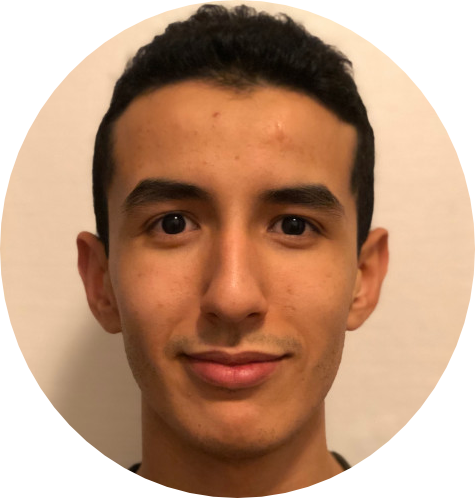
\includegraphics[width=0.1\textwidth]{Images/Team/MehdiABOUZAID.png} 
	\end{figure}
\end{textblock}

\begin{itemize}
\item[•] Article:
\item[] \textsl{Animal Recognition and Identification with Deep Convolutional Neural
Networks for Automated Wildlife Monitoring}
\item[•] Studied models:
\end{itemize}

\begin{adjustwidth}{-1.5em}{-1.5em}
\begin{center}
{\fontsize{9.5}{15}\selectfont
\begin{tabular}{|c|c|c|c|c|c|}
\cline{5-6}
\multicolumn{4}{c|}{} & \multicolumn{2}{c|}{\textit{Validation Set}} \\
\cline{2-6}
\multicolumn{1}{c|}{} & \textbf{ILSVRC} & \textbf{Parameters} & \textbf{Trainable Layers} & \textbf{Top-1 Accuracy} & \textbf{Top-5 Accuracy} \\
\hline
AlexNet & 2012 & 62,378,344 & 8 & 0.633 & 0.846 \\
\hline
VGG-16 & 2014 & 138,357,544 & 16 & 0.713 & 0.901 \\
\hline
ResNet-50 & 2015 & 25,636,712 & 50 & 0.749 & 0.921 \\
\hline
Xception & 2017 & 22,910,480 & 71 & 0.790 & 0.945 \\
\hline
\end{tabular}
}
\end{center}
\end{adjustwidth}

\begin{itemize}
\item[•] Vocabulary:
\item[] kernel = filter = receptive field = mask
\end{itemize}

\end{frame}

\subsection{Some information}
\begin{frame}
\frametitle{Introduction}
\framesubtitle{Our dataset} 

\begin{textblock}{15}(7.67,-0.62)
	\begin{figure}[H]
		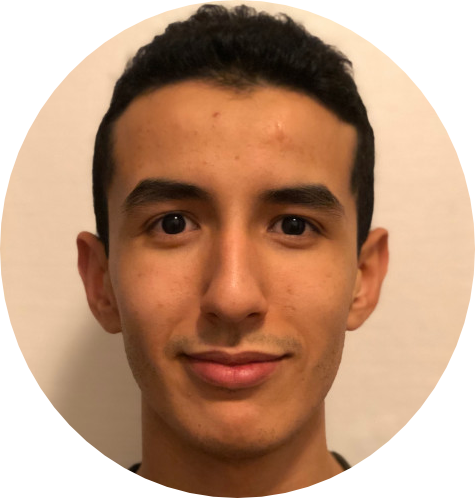
\includegraphics[width=0.1\textwidth]{Images/Team/MehdiABOUZAID.png} 
	\end{figure}
\end{textblock}

\setlength{\tabcolsep}{10pt} % spacing between columns
\begin{center}
\begin{tabular}{ccc}
\textbf{Input} & \textbf{Output} & \textbf{Number of Images} \\
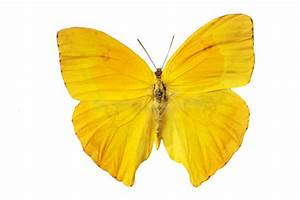
\includegraphics[valign=m,width=0.29\textwidth]{Images/Dataset/butterfly.jpeg} & butterfly & 1991 \\
\vspace{0.1cm}
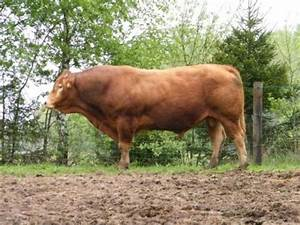
\includegraphics[valign=m,width=0.29\textwidth]{Images/Dataset/cow.jpeg} & cow & 2039 \\
\vspace{0.1cm}
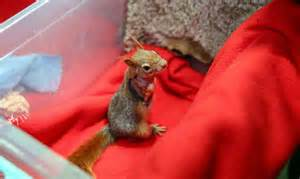
\includegraphics[valign=m,width=0.29\textwidth]{Images/Dataset/squirrel.jpeg} & squirrel & 2013  \\
\end{tabular}
\end{center}		 

\end{frame}